\documentclass[a4paper,hidelinks,14pt]{extarticle}

\usepackage[utf8]{inputenc}
\usepackage[T2A]{fontenc}
\usepackage[english, russian]{babel}
\usepackage{amsmath}
\usepackage{amssymb}
\usepackage{amsfonts}
\usepackage{mathtools}
\usepackage{datetime}
\usepackage[pdftex]{graphicx}
\usepackage{indentfirst}
\usepackage{asymptote}
\usepackage{systeme}
\usepackage[dvipsnames]{xcolor}
\usepackage{lastpage}
\usepackage{fancybox,fancyhdr}
\usepackage{hyperref}
\fancyhead[L]{Лабораторная работа №2}
\fancyhead[C]{}
\fancyhead[R]{Преобразование Фурье}
\fancyfoot[L]{}
\fancyfoot[C]{Страница \thepage\space из \pageref{LastPage}}
\fancyfoot[R]{}
\pagestyle{fancy}
\newcommand{\gt}{\textgreater}
\newcommand{\lt}{\textless}

\begin{document}
	\begin{titlepage}
		\setlength{\parindent}{0ex}
		
		\begin{center}
			\textsc{
				\vspace{1ex}
				Научно исследовательский университет ИТМО \\
				\vspace{0.5ex}
				Факультет систем управления и робототехники \\
				\vspace{0.5ex}
			}
		\end{center}
		
		\vspace{50mm}
		
		\begin{center}
			Отчет по лабораторной работе №2 \\
			Преобразование Фурье
		\end{center}
		
		\vspace{50mm}
		
		\begin{minipage}{.55\linewidth}
			Выполнил студент группы R3280
			
			Преподаватели
		\end{minipage}
		\hfill
		\begin{minipage}{.5\linewidth}
			\begin{flushright}
				Мовчан И. Е.
				\\
				Пашенко А.В., Перегудин А. А.
			\end{flushright}
		\end{minipage}
		
		\vfill
		\begin{center}
			Санкт-Петербург
			\\
			2024
		\end{center}
		
	\end{titlepage}
	
	\section{Вещественное}
	Будем рассматривать функции $f:\mathbb{R}\rightarrow\mathbb{R}$, а использовать унитарное преобразование Фурье к угловой частоте $\omega$, то есть
	$$
	f(t) = \frac{1}{\sqrt{2\pi}}\int\limits_{-\infty}^{\infty}\hat{f}(\omega) e^{i\omega t} d\omega,
	$$
	$$
	\hat{f}(\omega) = \frac{1}{\sqrt{2\pi}}\int\limits_{-\infty}^{\infty}f(t) e^{-i\omega t} dt,
	$$
	где $\hat{f}(\omega)$ задаёт Фурье-образ.
	
	\subsection{Прямоугольная функция}
	Функция имеет следующий вид:
	$
	f(t) =
	\left\{ 
	\begin{array}{l}
		a,\ |t| \le b, \\
		0,\ |t| > b.
	\end{array} 
	\right.
	$
	
	\vspace{1.25mm}
	Сразу отбросим очевидные случаи: 
	
	При $b < 0$ либо $a=0$ функция вырождается в тождественный ноль, то есть $f\equiv 0$ (очевидно, что тождественным нулём будет и её Фурье-образ)
	
	Для $b = 0$ иметь функцию, определённую только в одной точке ($t = 0$), но одна точка на значение интеграла никоим образом не влияет, а значит, Фурье-образ в этом случае тоже будет равен 0.
	
	В дальнейшем будем рассматривать именно ситуацию с $b > 0$ и $a \neq 0$ (наименее тривиальальный случай), когда функция будет иметь вид <<опущенного вниз>> (при $a < 0$) либо <<поднятого вверх>> (при $a > 0$) П-образного симметричного <<горбика>>.
	
	Найдём теперь Фурье-образ нашей функции:
	$$
	\hat{f}(\omega) = \frac{1}{\sqrt{2\pi}}\int\limits_{-b}^{b} a e^{-i\omega t}dt = -\frac{a}{\sqrt{2\pi}}\cdot\frac{e^{-i\omega t}}{i\omega} \bigg|_{t=-b}^{t=b}= \frac{a}{\sqrt{2\pi}}\cdot\frac{e^{i\omega b}-e^{-i\omega b}}{i\omega} = 
	$$
	
	$$
	= a\sqrt{\frac{2}{\pi}}\frac{\sin(\omega b)}{\omega} = ab\sqrt{\frac{2}{\pi}}\text{sinc}(\omega b)
	$$
	
	Параметр $ab$ в нашем случае отвечает за амплитуду колебаний графика Фурье-образа (чем он больше, тем выше <<размах>>, например, в 0), $b$ - за частоту (чем больше $b$, тем чаще происходят сами колебания).
	
	На рисунках \ref{1}, \ref{2} и \ref{3}  мы видим прямое подтверждение нашим выводам. Успех!
	\begin{figure}[h]
		\centering
		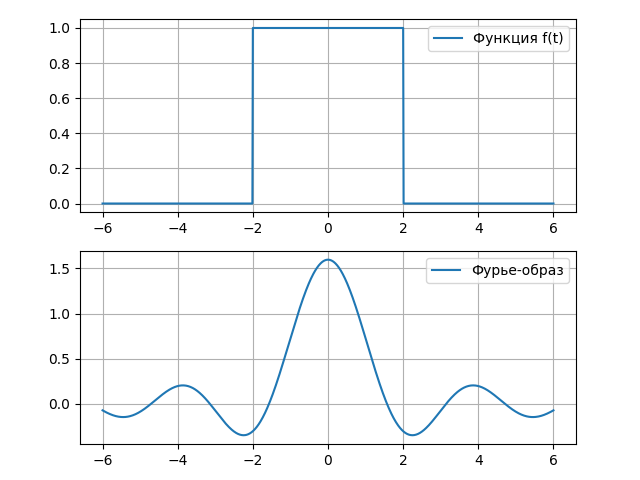
\includegraphics[scale=0.85]{images/Figure_1.png}
		\caption{Графики для значений $a = 1$, $b = 2$}
		\label{1}
	\end{figure}
	
	
	\begin{figure}[h]
		\centering
		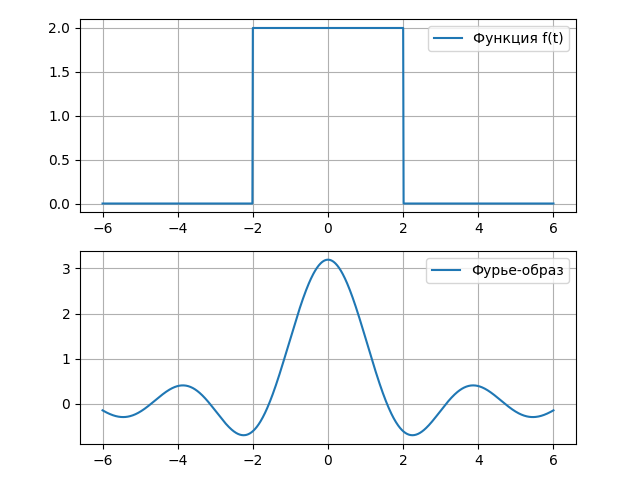
\includegraphics[scale=0.85]{images/Figure_2.png}
		\caption{Графики для значений $a = 2$, $b = 2$}
		\label{2}
	\end{figure}
	
	
	\begin{figure}[h]
		\centering
		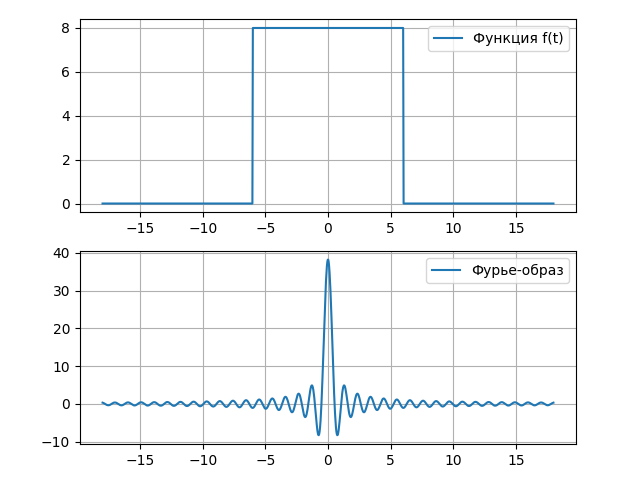
\includegraphics[scale=0.85]{images/Figure_3.png}
		\caption{Графики для значений $a = 8$, $b = 6$}
		\label{3}
	\end{figure}
	
	\subsection{Треугольная функция}
	Функция задана следующим образом:
	$
	f(t) =
	\left\{ 
	\begin{array}{l}
		a - |\frac{at}{b}|,\ |t| \le b, \\
		0,\ |t| > b.
	\end{array} 
	\right.
	$
	
	Здесь имеем аналогичные прошлому пункту особые случаи (с той лишь единственной разницей, что теперь $b \neq 0$). Так что сразу перейдём к выводу Фурье-образа:
	
	$$
	\hat{f}(\omega) = \frac{1}{\sqrt{2\pi}}\int\limits_{-b}^{b} (a - \left|\frac{at}{b}\right|) e^{-i\omega t}dt = ab\sqrt{\frac{2}{\pi}}\text{sinc}(\omega b) - \frac{1}{\sqrt{2\pi}}\int\limits_{-b}^{b} \left|\frac{at}{b}\right| e^{-i\omega t}dt =
	$$
	$$
	= ab\sqrt{\frac{2}{\pi}}\text{sinc}(\omega b) - \frac{1}{\sqrt{2\pi}}\int\limits_{0}^{b} \left|\frac{a}{b}\right|t e^{-i\omega t}dt + \frac{1}{\sqrt{2\pi}}\int\limits_{-b}^{0} \left|\frac{a}{b}\right|t e^{-i\omega t}dt =
	$$
	$$
	= ab\sqrt{\frac{2}{\pi}}\text{sinc}(\omega b) + \left|\frac{a}{b}\right|\cdot\frac{1}{\sqrt{2\pi}\omega^2}\left((i\omega t + 1)e^{-i\omega t}\bigg|_{-b}^0 - (i\omega t + 1)e^{-i\omega t}\bigg|_0^b\right)
	$$
	
	
	
	
	
	
	
	
	
	
	

\end{document}